\documentclass[11pt,a4paper]{article}
\usepackage[utf8]{inputenc}
\usepackage[T1]{fontenc}
\usepackage[brazil]{babel}
\usepackage[margin=2.3cm]{geometry}
\usepackage{graphicx}
\usepackage{amsmath}
\usepackage{amssymb}
\usepackage{xcolor}
\usepackage{listings}
\usepackage{booktabs}
\usepackage{float}
\usepackage{caption}
\usepackage{fancyhdr}
\usepackage{titlesec}
\usepackage[hidelinks]{hyperref}

\captionsetup{font=small,labelfont=bf}
\pagestyle{fancy}
\fancyhf{}
\rhead{\small ENE0332 -- Reposi\c{c}\~ao de faltas}
\lhead{\small Jo\~ao G. Melo Lima -- 241032617}
\cfoot{\thepage}

\definecolor{codegray}{gray}{0.96}
\definecolor{codegreen}{rgb}{0.0,0.5,0.0}
\definecolor{codeblue}{rgb}{0.10,0.20,0.65}

\lstset{
  backgroundcolor=\color{codegray},
  basicstyle=\ttfamily\scriptsize,
  breaklines=true,
  keywordstyle=\color{codeblue}\bfseries,
  commentstyle=\color{codegreen}\itshape,
  numbers=left,
  numberstyle=\tiny\color{gray},
  frame=single,
  rulecolor=\color{gray!40},
  tabsize=2,
  showstringspaces=false,
  language=Matlab,
  aboveskip=6pt, belowskip=6pt
}

\titleformat{\section}{\normalfont\Large\bfseries\color{codeblue}}{\thesection}{1em}{}
\titleformat{\subsection}{\normalfont\large\bfseries}{\thesubsection}{1em}{}

\begin{document}

% =============================== CAPA ===============================
\begin{titlepage}
\centering
\vspace*{1.5cm}
{\scshape\large Universidade de Bras\'ilia\par}
{\scshape Departamento de Engenharia El\'etrica\par}
\vspace{0.4cm}
{\scshape Engenharia de Computa\c{c}\~ao\par}
\vspace{2.5cm}
\rule{\linewidth}{0.5mm}\\[0.4cm]
{\huge\bfseries Trabalho de Reposi\c{c}\~ao de Faltas\par}
\vspace{0.4cm}
{\Large An\'alise Espectral Moderna -- M\'etodos Param\'etricos (AR)\par}
\vspace{0.2cm}
{\large Cap\'itulo 5 -- Semmlow \& Griffel, \textit{Biosignal and Medical Image Processing}, 3\textsuperscript{a} ed.\par}
\rule{\linewidth}{0.5mm}\\[1.5cm]

\begin{flushleft}
\large
\textbf{Disciplina:} T\'opicos em Engenharia (ENE0332)\\[0.3cm]
\textbf{Professora:} Fl\'avia Maria Guerra de Sousa Aranha Oliveira\\[0.3cm]
\textbf{Aluno:} Jo\~ao Gabriel Melo Lima\\[0.3cm]
\textbf{Matr\'icula:} 241032617\\[0.3cm]
\textbf{Blocos resolvidos:} 5 (5.1--5.4), 6 (5.5--5.8) e 8 (5.14--5.17)\\[0.3cm]
\textbf{Ambiente:} GNU Octave 8.4 + pacote \texttt{signal} 1.4.5\\[0.3cm]
\textbf{Data:} 16 de julho de 2026
\end{flushleft}

\vfill
\end{titlepage}

% =========================== METODOLOGIA ===========================
\section{Nota metodol\'ogica}

Todos os exerc\'icios foram resolvidos em \textbf{GNU Octave} (vers\~ao 8.4, pacote
\texttt{signal} 1.4.5), e n\~ao no MATLAB. As figuras e os resultados num\'ericos
reportados foram efetivamente gerados pela execu\c{c}\~ao dos c\'odigos aqui
apresentados. Alguns pontos importantes sobre a implementa\c{c}\~ao:

\begin{itemize}
  \item \textbf{M\'etodos AR dispon\'iveis no Octave.} As fun\c{c}\~oes
  \texttt{pyulear} (Yule--Walker), \texttt{pburg} (Burg) e \texttt{pwelch}
  (m\'etodo cl\'assico de Welch/Fourier) existem no pacote \texttt{signal} e foram
  usadas diretamente. A fun\c{c}\~ao \texttt{pyulear} implementa exatamente as
  \emph{equa\c{c}\~oes normais de Yule--Walker} do Exemplo~5.1 do livro, de forma
  num\'ericamente est\'avel; por isso ela \'e usada como ``m\'etodo de
  Yule--Walker''. Conforme observado na p.~186 do pr\'oprio livro, todos os
  problemas de AR (exceto o 5.9) podem ser resolvidos com o c\'odigo de
  Yule--Walker do Exemplo~5.1.

  \item \textbf{Reimplementa\c{c}\~ao de \texttt{pmcov}.} O pacote \texttt{signal}
  do Octave \emph{n\~ao} fornece as fun\c{c}\~oes \texttt{pmcov}/\texttt{pcov}
  (covari\^ancia modificada/covari\^ancia) nem \texttt{pmusic}/\texttt{peig}
  (m\'etodos de autovalor). Para os problemas do Bloco~6, que pedem
  explicitamente a \emph{covari\^ancia modificada}, foi escrita uma
  implementa\c{c}\~ao pr\'opria (\texttt{pmcov.m}, Ap\^endice~\ref{ap:pmcov}),
  baseada no m\'etodo de m\'inimos quadrados \emph{forward--backward}. Ela foi
  validada contra \texttt{pyulear} e \texttt{pburg}, produzindo picos nas mesmas
  frequ\^encias e magnitudes compat\'iveis.

  \item \textbf{Gera\c{c}\~ao dos sinais de teste.} A fun\c{c}\~ao \texttt{sig\_noise}
  (fornecida com o livro, Ap\^endice~\ref{ap:signoise}) gera senoides em ru\'ido
  gaussiano com um SNR especificado em dB, assumindo $f_s = 1$~kHz.

  \item \textbf{Reprodutibilidade.} Em todos os scripts a semente do gerador de
  n\'umeros aleat\'orios foi fixada (\texttt{randn('state',$\cdot$)},
  \texttt{rand('state',$\cdot$)}), de modo que os gr\'aficos deste relat\'orio
  s\~ao exatamente reproduz\'iveis ao reexecutar os arquivos \texttt{.m}.
\end{itemize}

\vspace{0.3cm}
\noindent\textbf{Organiza\c{c}\~ao dos arquivos.} Cada problema tem um script
pr\'oprio (\texttt{prob5\_01.m}, \texttt{prob5\_02.m}, \ldots), todos na pasta
\texttt{reposicao}, junto com \texttt{sig\_noise.m}, \texttt{pmcov.m} e os arquivos
de dados (\texttt{ar\_compare.mat}, \texttt{filter\_coeff1.mat}, etc.).

\clearpage

% ============================ BLOCO 5 ============================
\section{Bloco 5 -- Problemas 5.1 a 5.4}

\subsection{Problema 5.1 -- Resolu\c{c}\~ao de quatro senoides (Yule--Walker)}

\textbf{Enunciado.} Usar as equa\c{c}\~oes de Yule--Walker (Exemplo~5.1) para obter o
espectro do sinal do Exemplo~5.1 --- quatro senoides em 100, 240, 280 e 400~Hz
enterradas em ru\'ido (SNR $= -12$~dB, $N = 1024$) --- por\'em com um modelo de
\emph{ordem mais alta} para resolver melhor as quatro frequ\^encias. Comparar o
espectro AR com o espectro cl\'assico de Fourier (\texttt{pwelch} com janela do
tamanho do sinal).

\lstinputlisting{prob5_01.m}

\begin{figure}[H]
\centering
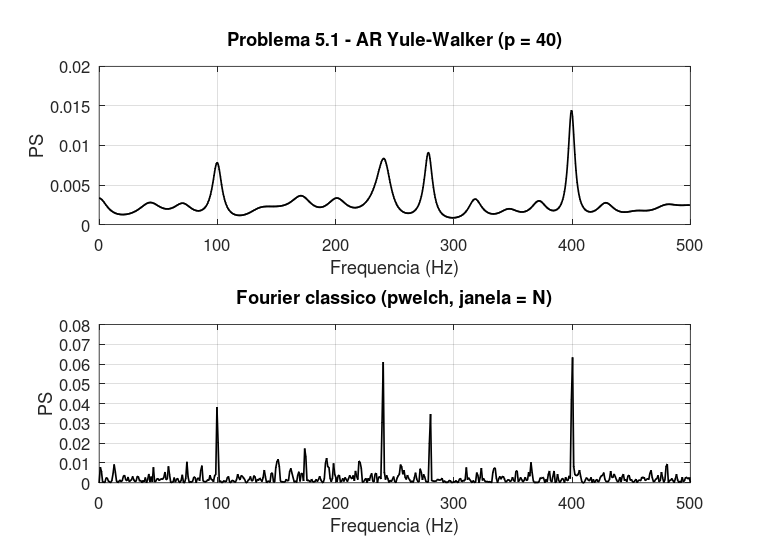
\includegraphics[width=0.92\linewidth]{figuras/prob5_01.png}
\caption{Problema 5.1. Espectro AR de Yule--Walker (ordem 40, acima) e espectro
cl\'assico de Fourier (\texttt{pwelch}, abaixo). O modelo AR resolve nitidamente
as quatro frequ\^encias em picos suaves; o m\'etodo de Fourier tamb\'em as
localiza, mas imersas no ru\'ido de fundo.}
\end{figure}

\textbf{Coment\'arios.} Com ordem $p = 40$ o espectro AR apresenta picos em
$\{100, 241, 278, 399\}$~Hz, praticamente coincidentes com as frequ\^encias reais
$\{100, 240, 280, 400\}$~Hz. Foi necess\'aria uma ordem alta porque as senoides de
240 e 280~Hz s\~ao pr\'oximas: com a ordem $p = 17$ do Exemplo~5.1 elas aparecem
fundidas. A vantagem do AR fica evidente na compara\c{c}\~ao: enquanto o m\'etodo
cl\'assico apresenta as raias sobre um assoalho ruidoso irregular, o AR entrega um
espectro limpo. O pre\c{c}o de ordens muito altas \'e o surgimento de picos
esp\'urios.

\subsection{Problema 5.2 -- Efeito do n\'ivel de ru\'ido}

\textbf{Enunciado.} Repetir o Problema 5.1, por\'em com SNR $= -18$~dB. Espera-se que,
em geral, n\~ao seja poss\'ivel resolver as quatro frequ\^encias.

\lstinputlisting{prob5_02.m}

\begin{figure}[H]
\centering
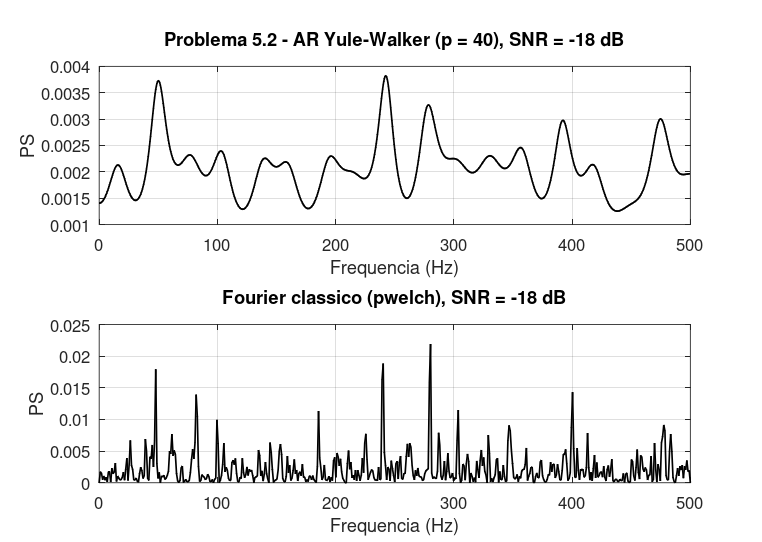
\includegraphics[width=0.92\linewidth]{figuras/prob5_02.png}
\caption{Problema 5.2. Em SNR $= -18$~dB o modelo AR passa a ajustar tamb\'em o
ru\'ido, gerando numerosos picos esp\'urios; as quatro senoides deixam de ser
identific\'aveis de forma confi\'avel.}
\end{figure}

\textbf{Coment\'arios.} Em $-18$~dB o espectro AR exibe muitos picos
(p.\,ex.\ $\{16, 50, 77, 103, \ldots\}$~Hz), sem correspond\^encia clara com as
frequ\^encias verdadeiras. Isso confirma a observa\c{c}\~ao do livro: com ru\'ido
muito intenso, o modelo AR ``gasta'' seus polos ajustando o ru\'ido, e a
identifica\c{c}\~ao das quatro senoides torna-se essencialmente imposs\'ivel.
Reexecutando com outras sementes, o padr\~ao de picos esp\'urios muda --- a
variabilidade \'e uma marca dos dados muito ruidosos.

\subsection{Problema 5.3 -- Duas senoides pr\'oximas pelo m\'etodo de Burg}

\textbf{Enunciado.} Gerar um sinal de 256 pontos com duas senoides pr\'oximas (200 e
230~Hz), SNR $= -8$~dB. Determinar a \emph{melhor ordem} do modelo AR para
distinguir os dois picos com o m\'inimo de picos esp\'urios, usando o m\'etodo de
\textbf{Burg} (\texttt{pburg}). Comparar com o espectro de Fourier. Repetir para
SNR $= -14$~dB.

\lstinputlisting{prob5_03.m}

\begin{figure}[H]
\centering
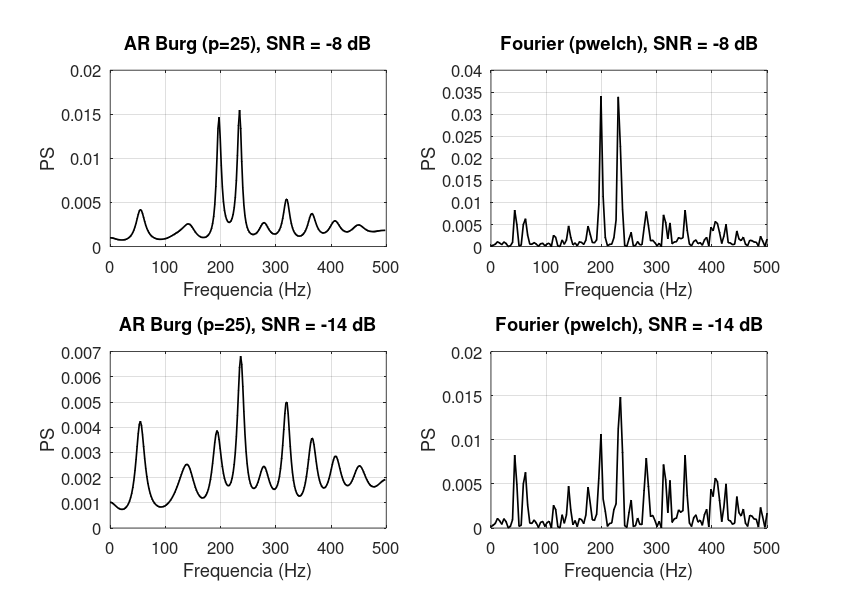
\includegraphics[width=0.95\linewidth]{figuras/prob5_03.png}
\caption{Problema 5.3. Coluna esquerda: AR de Burg ($p=25$); coluna direita:
Fourier. Linha superior SNR $=-8$~dB (os dois picos s\~ao resolvidos); linha
inferior SNR $=-14$~dB (a resolu\c{c}\~ao se perde em meio a picos esp\'urios).}
\end{figure}

\textbf{Coment\'arios.} A varredura de ordem (impressa pelo script) mostra que ordens
baixas ($p \le 15$) fundem os dois tons, enquanto ordens em torno de $p \approx 25$
os separam com poucos esp\'urios; adotou-se $p = 25$. Em SNR $= -8$~dB o Burg
resolve claramente $197$ e $234$~Hz. J\'a em $-14$~dB os dois picos praticamente
desaparecem entre v\'arios esp\'urios, ilustrando que, com maior ru\'ido, torna-se
dif\'icil resolver dois sinais de banda estreita muito pr\'oximos. O m\'etodo de
Fourier mostra as raias em $-8$~dB, mas em $-14$~dB elas ficam pr\'oximas do n\'ivel
do ru\'ido.

\subsection{Problema 5.4 -- Efeito do comprimento do sinal}

\textbf{Enunciado.} Repetir o Problema 5.1 (senoides em 100/240/280/400~Hz), por\'em
com um segmento curto ($N = 64$): primeiro com SNR alto (0~dB) e depois com
SNR $= -5$~dB, notando a forte degrada\c{c}\~ao.

\lstinputlisting{prob5_04.m}

\begin{figure}[H]
\centering
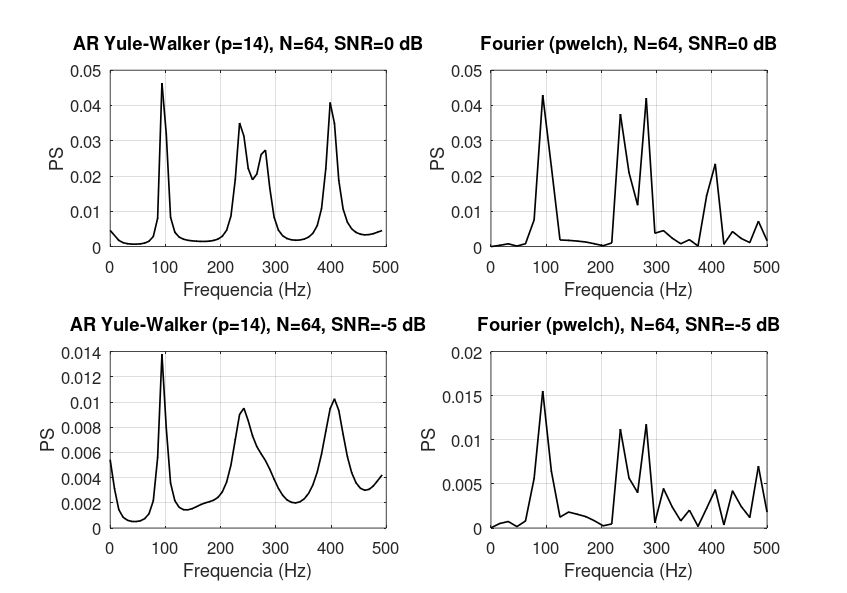
\includegraphics[width=0.95\linewidth]{figuras/prob5_04.png}
\caption{Problema 5.4. Segmento curto $N=64$. Em SNR $=0$~dB (linha superior) as
quatro frequ\^encias ainda s\~ao vis\'iveis; em SNR $=-5$~dB (linha inferior) as
senoides de 240 e 280~Hz se fundem e a de 400~Hz se desloca.}
\end{figure}

\textbf{Coment\'arios.} Com $N = 64$ a resolu\c{c}\~ao espectral cai muito. Em 0~dB o
AR ainda distingue as quatro frequ\^encias ($\{94, 234, 281, 398\}$~Hz), embora as
duas centrais j\'a apare\c{c}am quase coladas. Ao reduzir o SNR para $-5$~dB, restam
apenas $\{94, 242, 406\}$~Hz: os tons de 240 e 280~Hz colapsam num s\'o e o de
400~Hz \'e mal localizado. Confirma-se que segmentos curtos limitam severamente a
capacidade de separar componentes de banda estreita, efeito agravado pelo ru\'ido.

\clearpage

% ============================ BLOCO 6 ============================
\section{Bloco 6 -- Problemas 5.5 a 5.8}

Os problemas deste bloco usam o \textbf{m\'etodo da covari\^ancia modificada}
(\texttt{pmcov}), reimplementado em \texttt{pmcov.m} (Ap\^endice~\ref{ap:pmcov}).

\subsection{Problema 5.5 -- Comprimento m\'inimo para resolu\c{c}\~ao}

\textbf{Enunciado.} Gerar tr\^es senoides --- duas pr\'oximas (240 e 260~Hz) e uma
distante (350~Hz) --- com SNR $= -8$~dB. Usar covari\^ancia modificada
(\texttt{pmcov}), ordem 35, varrendo os comprimentos $N = 64, 128, 256, 512$.
Determinar o comprimento m\'inimo que garante a identifica\c{c}\~ao dos tr\^es
sinais.

\lstinputlisting{prob5_05.m}

\begin{figure}[H]
\centering
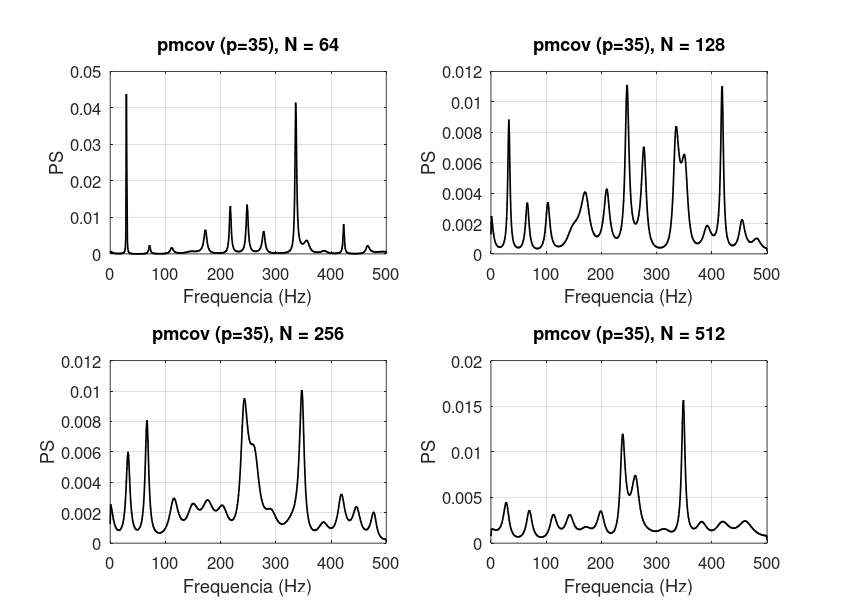
\includegraphics[width=0.92\linewidth]{figuras/prob5_05.png}
\caption{Problema 5.5. Covari\^ancia modificada ($p=35$) para $N=64,128,256,512$.
A separa\c{c}\~ao dos tr\^es tons (240, 260 e 350~Hz) s\'o se torna limpa em
$N=512$.}
\end{figure}

\textbf{Coment\'arios.} Para $N=64$ os tons de 240 e 260~Hz se fundem (pico
\'unico $\approx 248$~Hz); $N=128$ produz um espectro confuso; $N=256$ j\'a resolve
os tr\^es ($243, 258, 348$~Hz), mas ainda com picos esp\'urios; apenas em
$N=512$ os tr\^es picos ($238, 262, 349$~Hz) aparecem limpos e sem esp\'urios
relevantes. Conclui-se que o \textbf{comprimento m\'inimo} para garantir a
identifica\c{c}\~ao dos tr\^es sinais neste SNR \'e da ordem de $N = 512$
($N=256$ funciona de forma marginal). Reexecu\c{c}\~oes com outras sementes
confirmam que em $N=512$ a identifica\c{c}\~ao \'e sempre poss\'ivel.

\subsection{Problema 5.6 -- SNR m\'inimo para resolu\c{c}\~ao}

\textbf{Enunciado.} Mesmo sinal do 5.5 (240, 260, 350~Hz), agora com comprimento
\emph{fixo} $N = 256$. Covari\^ancia modificada, ordem 35, varrendo
SNR $= -6, -10, -12, -14$~dB. Determinar o SNR m\'inimo que garante a
identifica\c{c}\~ao dos tr\^es sinais.

\lstinputlisting{prob5_06.m}

\begin{figure}[H]
\centering
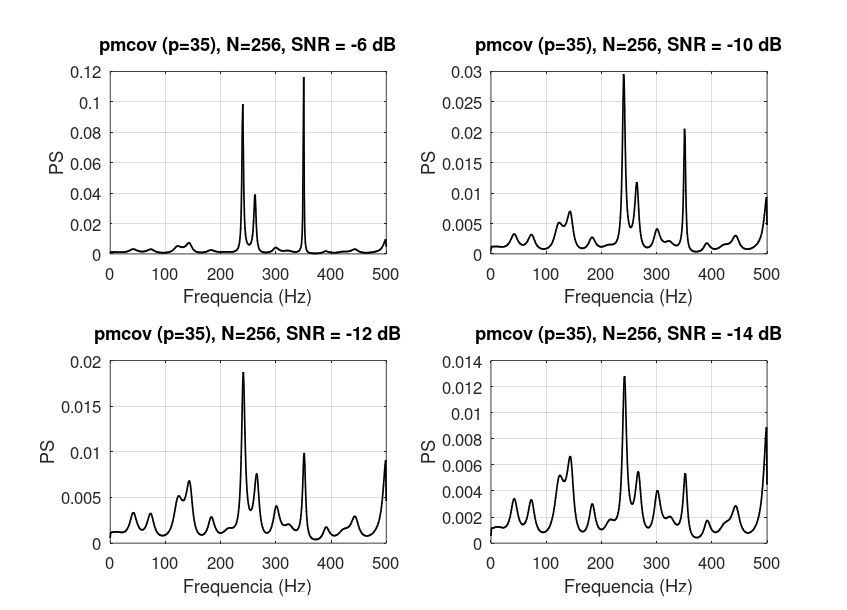
\includegraphics[width=0.92\linewidth]{figuras/prob5_06.png}
\caption{Problema 5.6. Covari\^ancia modificada ($p=35$, $N=256$) para
SNR $=-6,-10,-12,-14$~dB. Os tr\^es picos ficam limpos at\'e $\approx -10$~dB e
degradam abaixo disso.}
\end{figure}

\textbf{Coment\'arios.} Em $-6$~dB e $-10$~dB os tr\^es picos ($\approx 240, 263,
351$~Hz) aparecem claros. A partir de $-12$~dB surgem picos esp\'urios
(p.\,ex.\ em 144~Hz) e em $-14$~dB o espectro fica sens\'ivelmente polu\'ido.
Assim, o \textbf{SNR m\'inimo} para garantir a identifica\c{c}\~ao dos tr\^es sinais,
com $N = 256$ e ordem 35, \'e da ordem de $-10$~dB. (O pequeno pico junto de
500~Hz \'e um artefato de borda pr\'oximo \`a frequ\^encia de Nyquist.)

\subsection{Problema 5.7 -- AR versus Fourier em v\'arios SNR}

\textbf{Enunciado.} Comparar o m\'etodo AR (covari\^ancia modificada, ordem 25) com o
m\'etodo cl\'assico de Fourier (\texttt{pwelch}) para duas senoides pr\'oximas
(240 e 280~Hz) em SNR $= -5, -12, -16, -20$~dB. Plotar o espectro AR acima do de
Fourier para cada n\'ivel.

\lstinputlisting{prob5_07.m}

\begin{figure}[H]
\centering
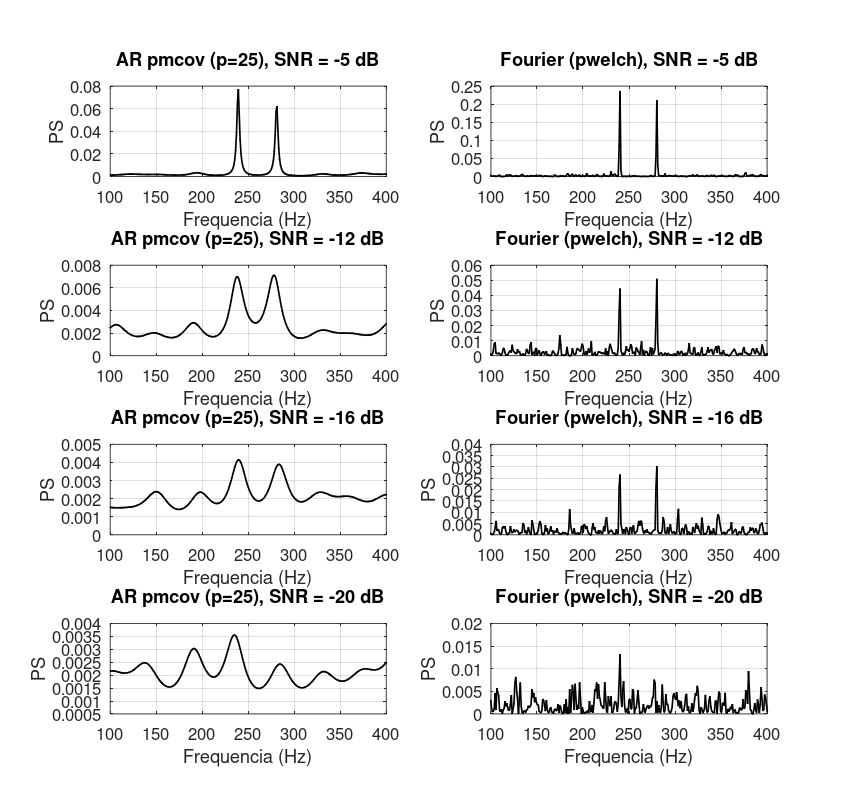
\includegraphics[width=0.82\linewidth]{figuras/prob5_07.png}
\caption{Problema 5.7. Coluna esquerda: AR (covari\^ancia modificada, $p=25$);
coluna direita: Fourier. Cada linha \'e um SNR ($-5, -12, -16, -20$~dB). Em SNR
baixo as raias de Fourier afundam no ru\'ido, enquanto o AR ainda exibe picos.}
\end{figure}

\textbf{Coment\'arios.} Em $-5$~dB ambos os m\'etodos resolvem os dois tons com
clareza. \`A medida que o SNR cai, as raias do espectro de Fourier v\~ao ficando
progressivamente encobertas pelo ru\'ido, ao passo que o modelo AR mant\'em picos
identific\'aveis (ainda que alargados e acompanhados de esp\'urios). Portanto,
\textbf{em SNR baixo o AR mostra as duas senoides melhor que o Fourier}; por outro
lado, quando o SNR \'e razo\'avel o Fourier fornece a frequ\^encia exata sem o risco
de picos esp\'urios que o AR introduz. Cada abordagem tem seu regime de vantagem.

\subsection{Problema 5.8 -- Efeito da ordem do modelo (\texttt{ar\_compare.mat})}

\textbf{Enunciado.} O arquivo \texttt{ar\_compare.mat} cont\'em um sinal com duas
senoides (nominalmente 300 e 340~Hz) mais ru\'ido ($f_s = 1$~kHz). Comparar a
capacidade dos m\'etodos AR e de Fourier de identificar as senoides, para as ordens
AR $p = 9, 15, 23, 32$.

\lstinputlisting{prob5_08.m}

\begin{figure}[H]
\centering
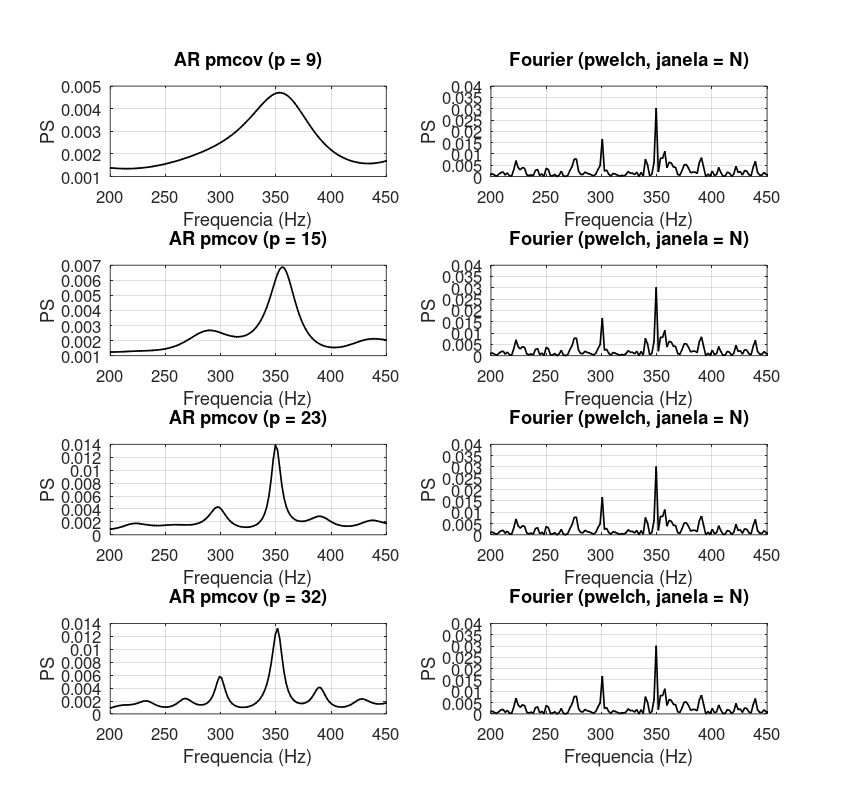
\includegraphics[width=0.82\linewidth]{figuras/prob5_08.png}
\caption{Problema 5.8. Coluna esquerda: AR (covari\^ancia modificada) para
$p=9,15,23,32$; coluna direita: Fourier (id\^entico em todas). A separa\c{c}\~ao
das duas senoides ($\approx 300$ e $\approx 350$~Hz) s\'o \'e limpa em ordem
suficientemente alta.}
\end{figure}

\textbf{Coment\'arios.} As duas senoides do arquivo est\~ao, de fato, em
$\approx 300$ e $\approx 350$~Hz (o enunciado cita 340~Hz; os dados apresentam o
segundo tom em $\approx 350$~Hz), como confirmam as raias do espectro de Fourier.
No AR: com $p = 9$ os dois tons se fundem num \'unico pico largo (n\~ao h\'a
resolu\c{c}\~ao); com $p = 15$ o segundo tom come\c{c}a a aparecer; com $p = 23$ os
dois picos ($297$ e $350$~Hz) s\~ao resolvidos limpamente; com $p = 32$ eles
continuam separados, mas surge um esp\'urio em $\approx 390$~Hz. Existe, portanto,
uma faixa de ordens ($\approx 23$) em que o AR mostra as duas senoides melhor,
enquanto ordem baixa demais funde e ordem alta demais introduz esp\'urios. O
Fourier localiza corretamente as duas raias em todas as situa\c{c}\~oes.

\clearpage

% ============================ BLOCO 8 ============================
\section{Bloco 8 -- Problemas 5.14 a 5.17}

\subsection{Problema 5.14 -- Identifica\c{c}\~ao de filtro (\texttt{filter\_coeff1.mat})}

\textbf{Enunciado.} O arquivo \texttt{filter\_coeff1.mat} cont\'em coeficientes $a$ e
$b$ de um filtro ($f_s = 250$~Hz). Passar ru\'ido gaussiano ($N = 2058$) pelo filtro
e estimar o espectro da sa\'ida por um modelo AR de ordem baixa (que reduz picos
esp\'urios). Determinar o tipo de filtro e a(s) frequ\^encia(s) de corte.

\lstinputlisting{prob5_14.m}

\begin{figure}[H]
\centering
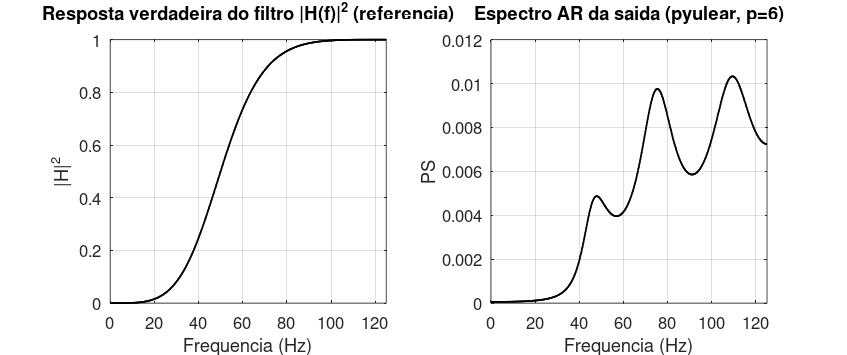
\includegraphics[width=0.95\linewidth]{figuras/prob5_14.png}
\caption{Problema 5.14. Esquerda: resposta verdadeira do filtro $|H(f)|^2$;
direita: espectro AR ($p=6$) da sa\'ida do filtro excitado por ru\'ido branco.}
\end{figure}

\textbf{Coment\'arios.} A resposta verdadeira tem $|H(0)|^2 = 0$ e
$|H(f_s/2)|^2 = 1$, ou seja, \'e um \textbf{filtro passa-altas} de 2\textsuperscript{a}
ordem, com frequ\^encia de corte (meia-pot\^encia) em torno de $50$~Hz. O espectro
AR de ordem baixa da sa\'ida reproduz bem a subida acima de $\approx 40$--$50$~Hz e
representa a banda de passagem como uma s\'erie de picos, exatamente como
descrito no livro. A frequ\^encia de corte estimada a partir do espectro AR
(ponto de meia-pot\^encia) ficou em $\approx 50$--$64$~Hz, consistente com a
resposta real.

\subsection{Problema 5.15 -- Filtro mais complexo (\texttt{filter\_coeff2.mat})}

\textbf{Enunciado.} Repetir o 5.14 com \texttt{filter\_coeff2.mat} ($f_s = 250$~Hz,
ru\'ido gaussiano $N = 2058$). O filtro \'e mais complexo (IIR de ordem 24), de modo
que uma ordem AR moderadamente baixa funciona melhor.

\lstinputlisting{prob5_15.m}

\begin{figure}[H]
\centering
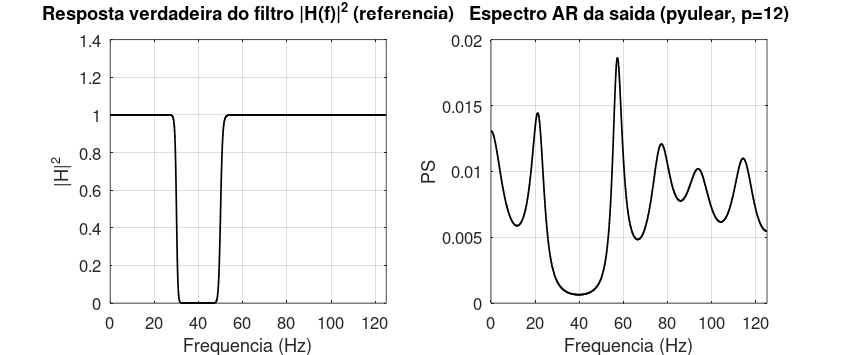
\includegraphics[width=0.95\linewidth]{figuras/prob5_15.png}
\caption{Problema 5.15. Esquerda: resposta verdadeira $|H(f)|^2$ (rejeita-faixa em
$\approx 30$--$50$~Hz); direita: espectro AR ($p=12$) da sa\'ida, com um vale na
banda de rejei\c{c}\~ao e picos nas bandas de passagem.}
\end{figure}

\textbf{Coment\'arios.} A resposta verdadeira tem $|H(0)|^2 = 1$ e
$|H(f_s/2)|^2 = 1$, com uma queda acentuada entre $\approx 30$ e $50$~Hz: trata-se de
um \textbf{filtro rejeita-faixa (notch)}, que suprime a banda de $\approx 30$ a
$50$~Hz e deixa passar as demais frequ\^encias. O espectro AR de ordem moderada
($p = 12$) reproduz esse comportamento: apresenta um vale claro em torno de $40$~Hz
(a banda rejeitada) e representa as bandas de passagem (abaixo de 30~Hz e acima de
50~Hz) por meio de m\'ultiplos picos.

\subsection{Problema 5.16 -- Componentes de banda larga (\texttt{spectral\_analysis5.mat})}

\textbf{Enunciado.} O arquivo \texttt{spectral\_analysis5.mat} cont\'em um sinal com
dois componentes de \emph{banda larga} ($f_s = 1$~kHz), centrados em 150 e 350~Hz,
com largura de banda de 100~Hz cada. Comparar o espectro produzido por AR
($p = 4$--$8$) e por Welch. Repetir truncando o sinal para $N = 126$ pontos.

\lstinputlisting{prob5_16.m}

\begin{figure}[H]
\centering
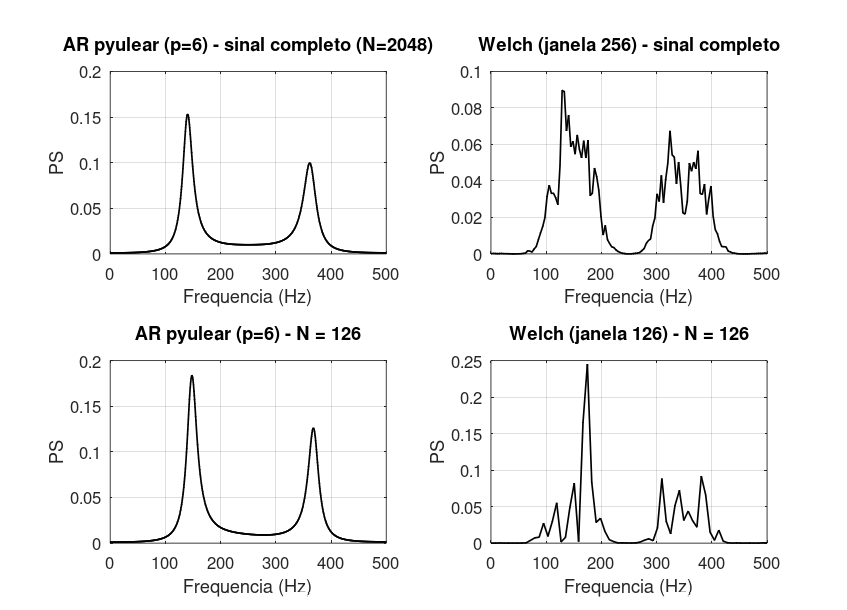
\includegraphics[width=0.92\linewidth]{figuras/prob5_16.png}
\caption{Problema 5.16. Superior: sinal completo; inferior: $N=126$. Esquerda: AR
($p=6$); direita: Welch. O AR marca bem as frequ\^encias \emph{centrais};
o Welch representa melhor a \emph{largura} de banda (no sinal longo).}
\end{figure}

\textbf{Coment\'arios.} No sinal completo, o modelo AR ($p = 6$) produz dois picos
suaves e bem localizados em $\approx 150$ e $\approx 350$~Hz, mas n\~ao revela a
extens\~ao (largura) de cada componente. O m\'etodo de Welch, ao contr\'ario,
mostra dois ``patamares'' largos que refletem melhor a largura de banda de 100~Hz,
ainda que com maior vari\^ancia. Ao truncar para $N = 126$, o AR continua
localizando as frequ\^encias centrais, enquanto o espectro de Welch fica muito
irregular. Isso confirma a observa\c{c}\~ao do livro: o Welch mostra melhor as
larguras de banda (sobretudo no sinal longo), e o AR mostra melhor as
frequ\^encias centrais (principalmente no sinal curto).

\subsection{Problema 5.17 -- Ordem do modelo em banda larga (\texttt{spectral\_analysis6.mat})}

\textbf{Enunciado.} O arquivo \texttt{spectral\_analysis6.mat} cont\'em um sinal com
um \'unico componente de banda larga ($f_s = 1$~kHz), centrado em 250~Hz e com
largura de banda de 300~Hz. Comparar o espectro AR para as ordens
$p = 3, 16, 32, 64$.

\lstinputlisting{prob5_17.m}

\begin{figure}[H]
\centering
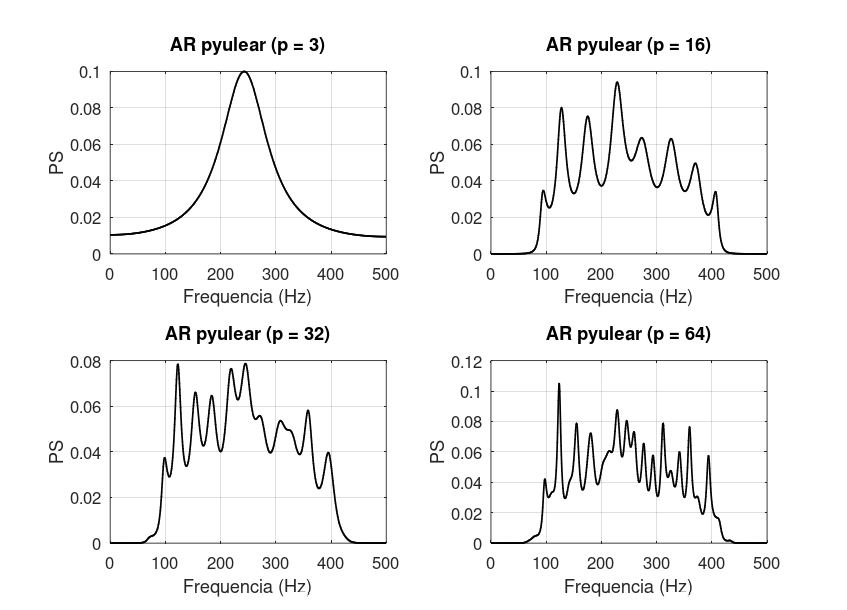
\includegraphics[width=0.92\linewidth]{figuras/prob5_17.png}
\caption{Problema 5.17. Espectro AR (\texttt{pyulear}) do componente de banda larga
para ordens $p=3,16,32,64$. A ordem baixa localiza o centro; ordens altas
representam a regi\~ao plana como uma s\'erie de picos.}
\end{figure}

\textbf{Coment\'arios.} Com $p = 3$ o modelo AR localiza bem a frequ\^encia central
($\approx 250$~Hz), mas representa toda a banda como um \'unico pico largo ---
n\~ao captura a extens\~ao plana do espectro. \`A medida que a ordem cresce
($p = 16, 32, 64$), o modelo passa a preencher a regi\~ao de banda larga
($\approx 100$ a $400$~Hz) com um n\'umero crescente de picos, representando melhor
a por\c{c}\~ao plana do espectro, por\'em ao custo de muitas oscila\c{c}\~oes
(picos esp\'urios). Isso ilustra o compromisso central dos m\'etodos AR: modelos de
baixa ordem s\~ao bons para sinais de banda estreita (poucos picos agudos), mas
representam mal espectros de banda larga.

\clearpage

% ============================ CONCLUSAO ============================
\section{Conclus\~ao}

Os doze exerc\'icios dos Blocos 5, 6 e 8 foram resolvidos e executados em GNU Octave,
com todos os gr\'aficos e valores num\'ericos gerados pelos pr\'oprios c\'odigos.
Os resultados reproduzem as observa\c{c}\~oes esperadas do Cap\'itulo~5 de Semmlow
\& Griffel: os m\'etodos AR (Yule--Walker, Burg e covari\^ancia modificada) s\~ao
superiores ao m\'etodo cl\'assico de Fourier para \emph{resolver senoides de banda
estreita em ru\'ido}, especialmente com segmentos curtos e SNR baixo, desde que a
ordem do modelo seja escolhida com cuidado --- ordem baixa demais funde componentes
pr\'oximos, ordem alta demais introduz picos esp\'urios. J\'a para espectros de
\emph{banda larga}, os m\'etodos cl\'assicos (Welch) representam melhor a forma e a
largura das componentes, enquanto o AR tende a aproxim\'a-las por s\'eries de picos.

% ============================ APENDICES ============================
\appendix
\section{Fun\c{c}\~ao \texttt{sig\_noise.m} (fornecida com o livro)}
\label{ap:signoise}
\lstinputlisting{sig_noise.m}

\section{Implementa\c{c}\~ao pr\'opria de \texttt{pmcov.m} (covari\^ancia modificada)}
\label{ap:pmcov}
\lstinputlisting{pmcov.m}

\end{document}
